\chapter{Architecture}\label{ch:arch}

The application is compound of three components:
\begin{enumerate*}[label=]
	\item Scraper;
	\item Server;
	\item Client.
\end{enumerate*}
A library (DataModel) is used by the Server and the Scraper to access the
database. Server and Client exchange messages using a Common library.

\begin{figure}[p]
	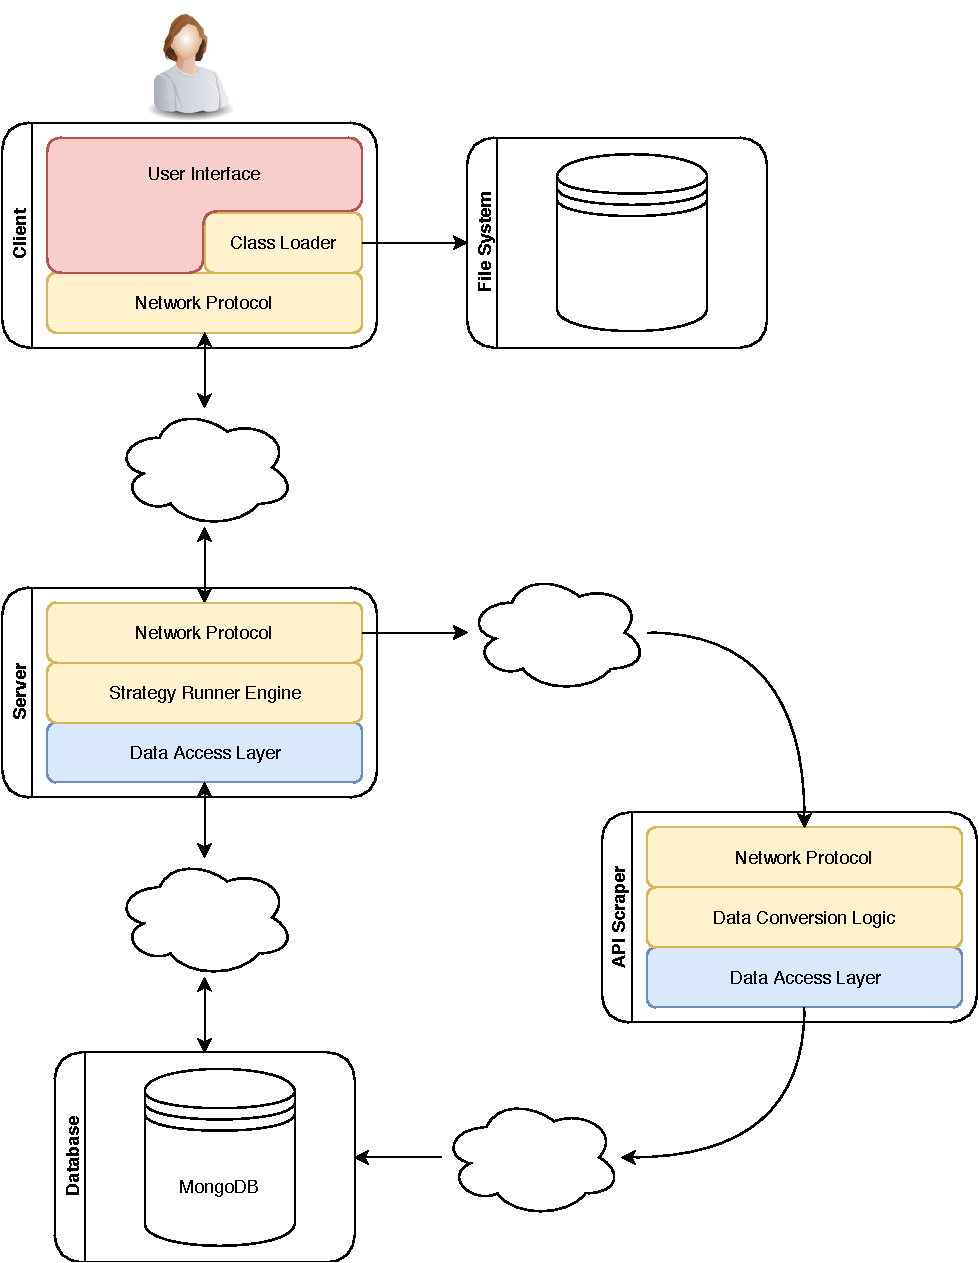
\includegraphics[width=\textwidth]{arch}
	\caption{Application architecture.}\label{fig:arch}
\end{figure}

\figref{fig:arch} shows the application's architecture.

\section{Scraper}\label{sec:scraper}

This is the application that downloads data from the configured sources (Binance
and Coinbase).

The \code{net} package contains the classes used to call the sources' API\@. It
uses the \code{Retrofit} library to build the HTTP requests. The API responds
with JSON documents that are deserialized using the \code{Gson} library.

The main work is done by the \code{Worker} class: the scraper starts a thread
for each source and each of these threads cycles over all the markets configured
for its data source to download the market data.

The scraper also listen on a socket in order to get commands from the server
application that instruct the scraper to restart itself (and reload the
configuration from the database). This happens every time the administrator
changes the configuration for a source or a market.

\begin{landscape}
	\begin{figure}[!ht]
		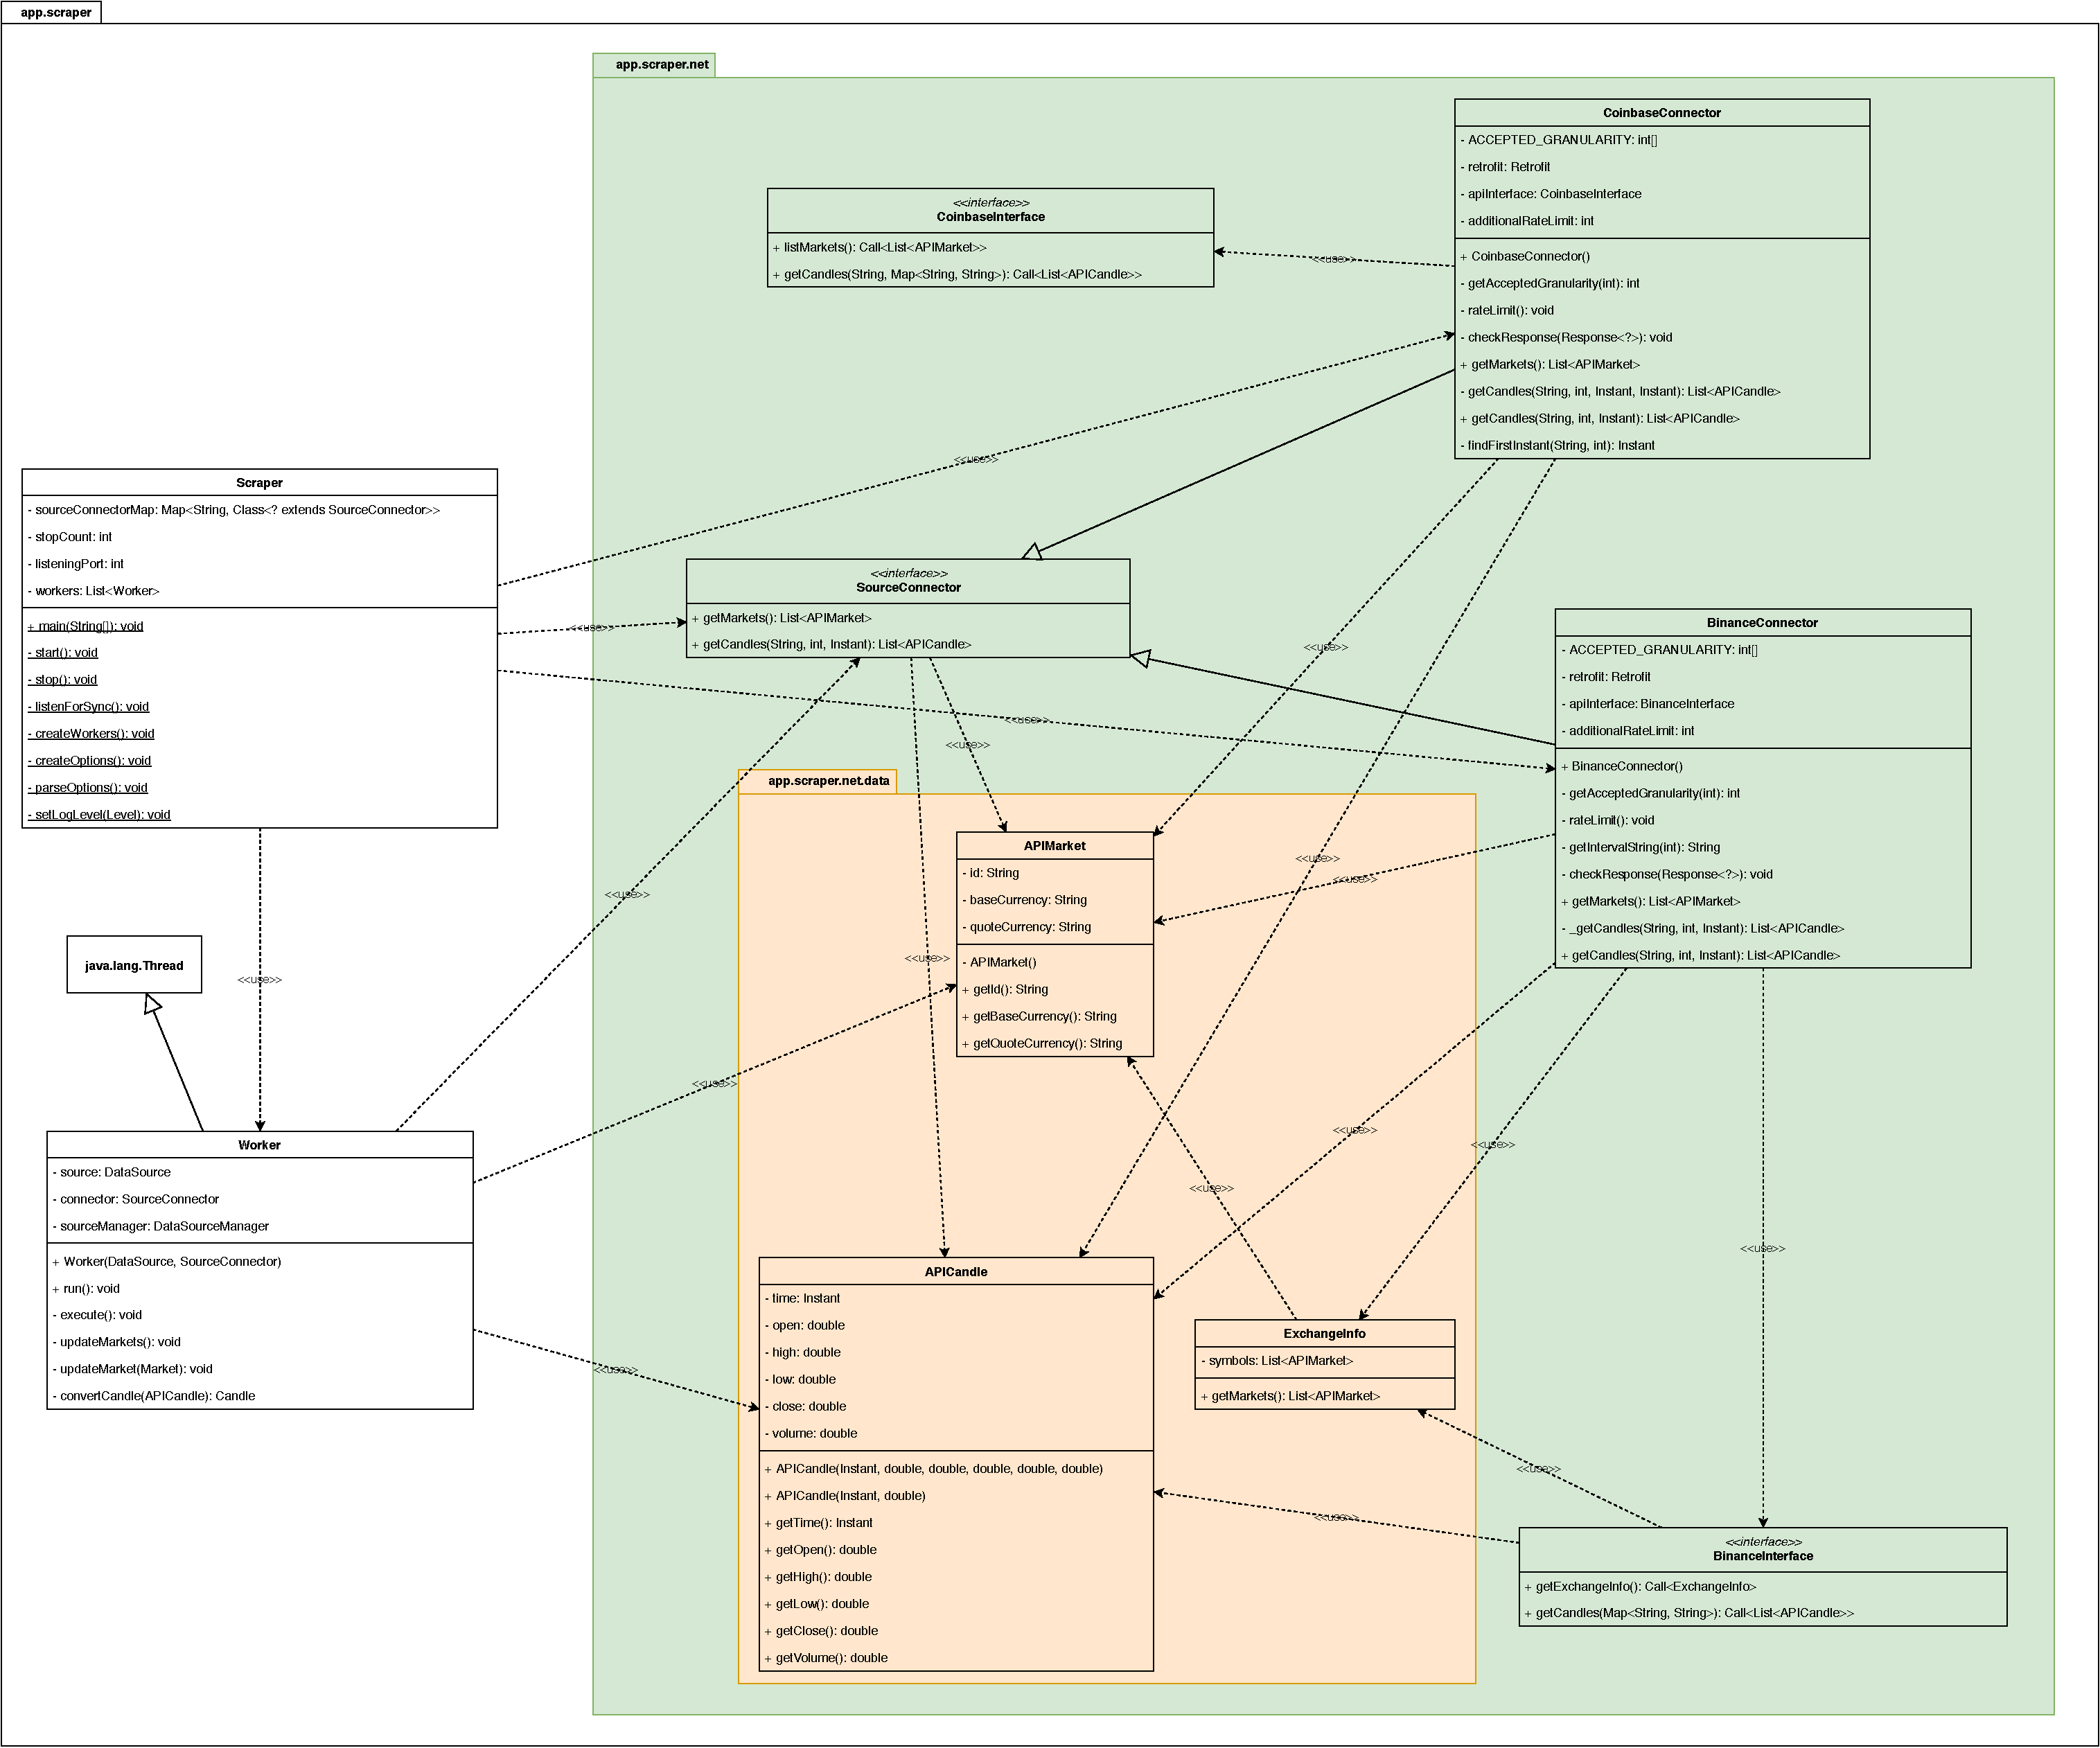
\includegraphics[width=0.7\paperheight]{module-scraper}
		\caption*{\textbf{Figure~\ref{fig:scraper}}}
		\captionlistentry{}\label{fig:scraper}
	\end{figure}
\end{landscape}

\section{Server}\label{sec:server}

The server application implements the main business logic of the system.

For each request received a new thread to handle the request is started
(stateless server). First, when a new request arrive, the application checks if
the user has the right privilege to run the request operation and if the message
is valid \idest{contains all the required entities}. Then the appropriate
request handler is called. The request handler perform the requested operation
(that usually involves in loading some data from the database, edit it and then
save it back to the database) and generate the response that must be sent back
to the client.

The most complex part is the one in the \code{app.server.runner} package. Here
are contained the classes used to load/save the strategies from/to the file
system and to run the strategies over the market data.

The strategy execution is handled by the \code{StrategyRunner} class. The
aggregation pipeline used to get the data needed to run the strategy is built by
the \code{AggregationRunner} class. Note that the aggregation pipeline is not
always the same: it changes based on which indicators are used by the strategy.
The pipeline stages needed by each indicator are returned by the
\code{pipeline()} method of the indicators' classes.

\begin{landscape}
	\begin{figure}[!ht]
		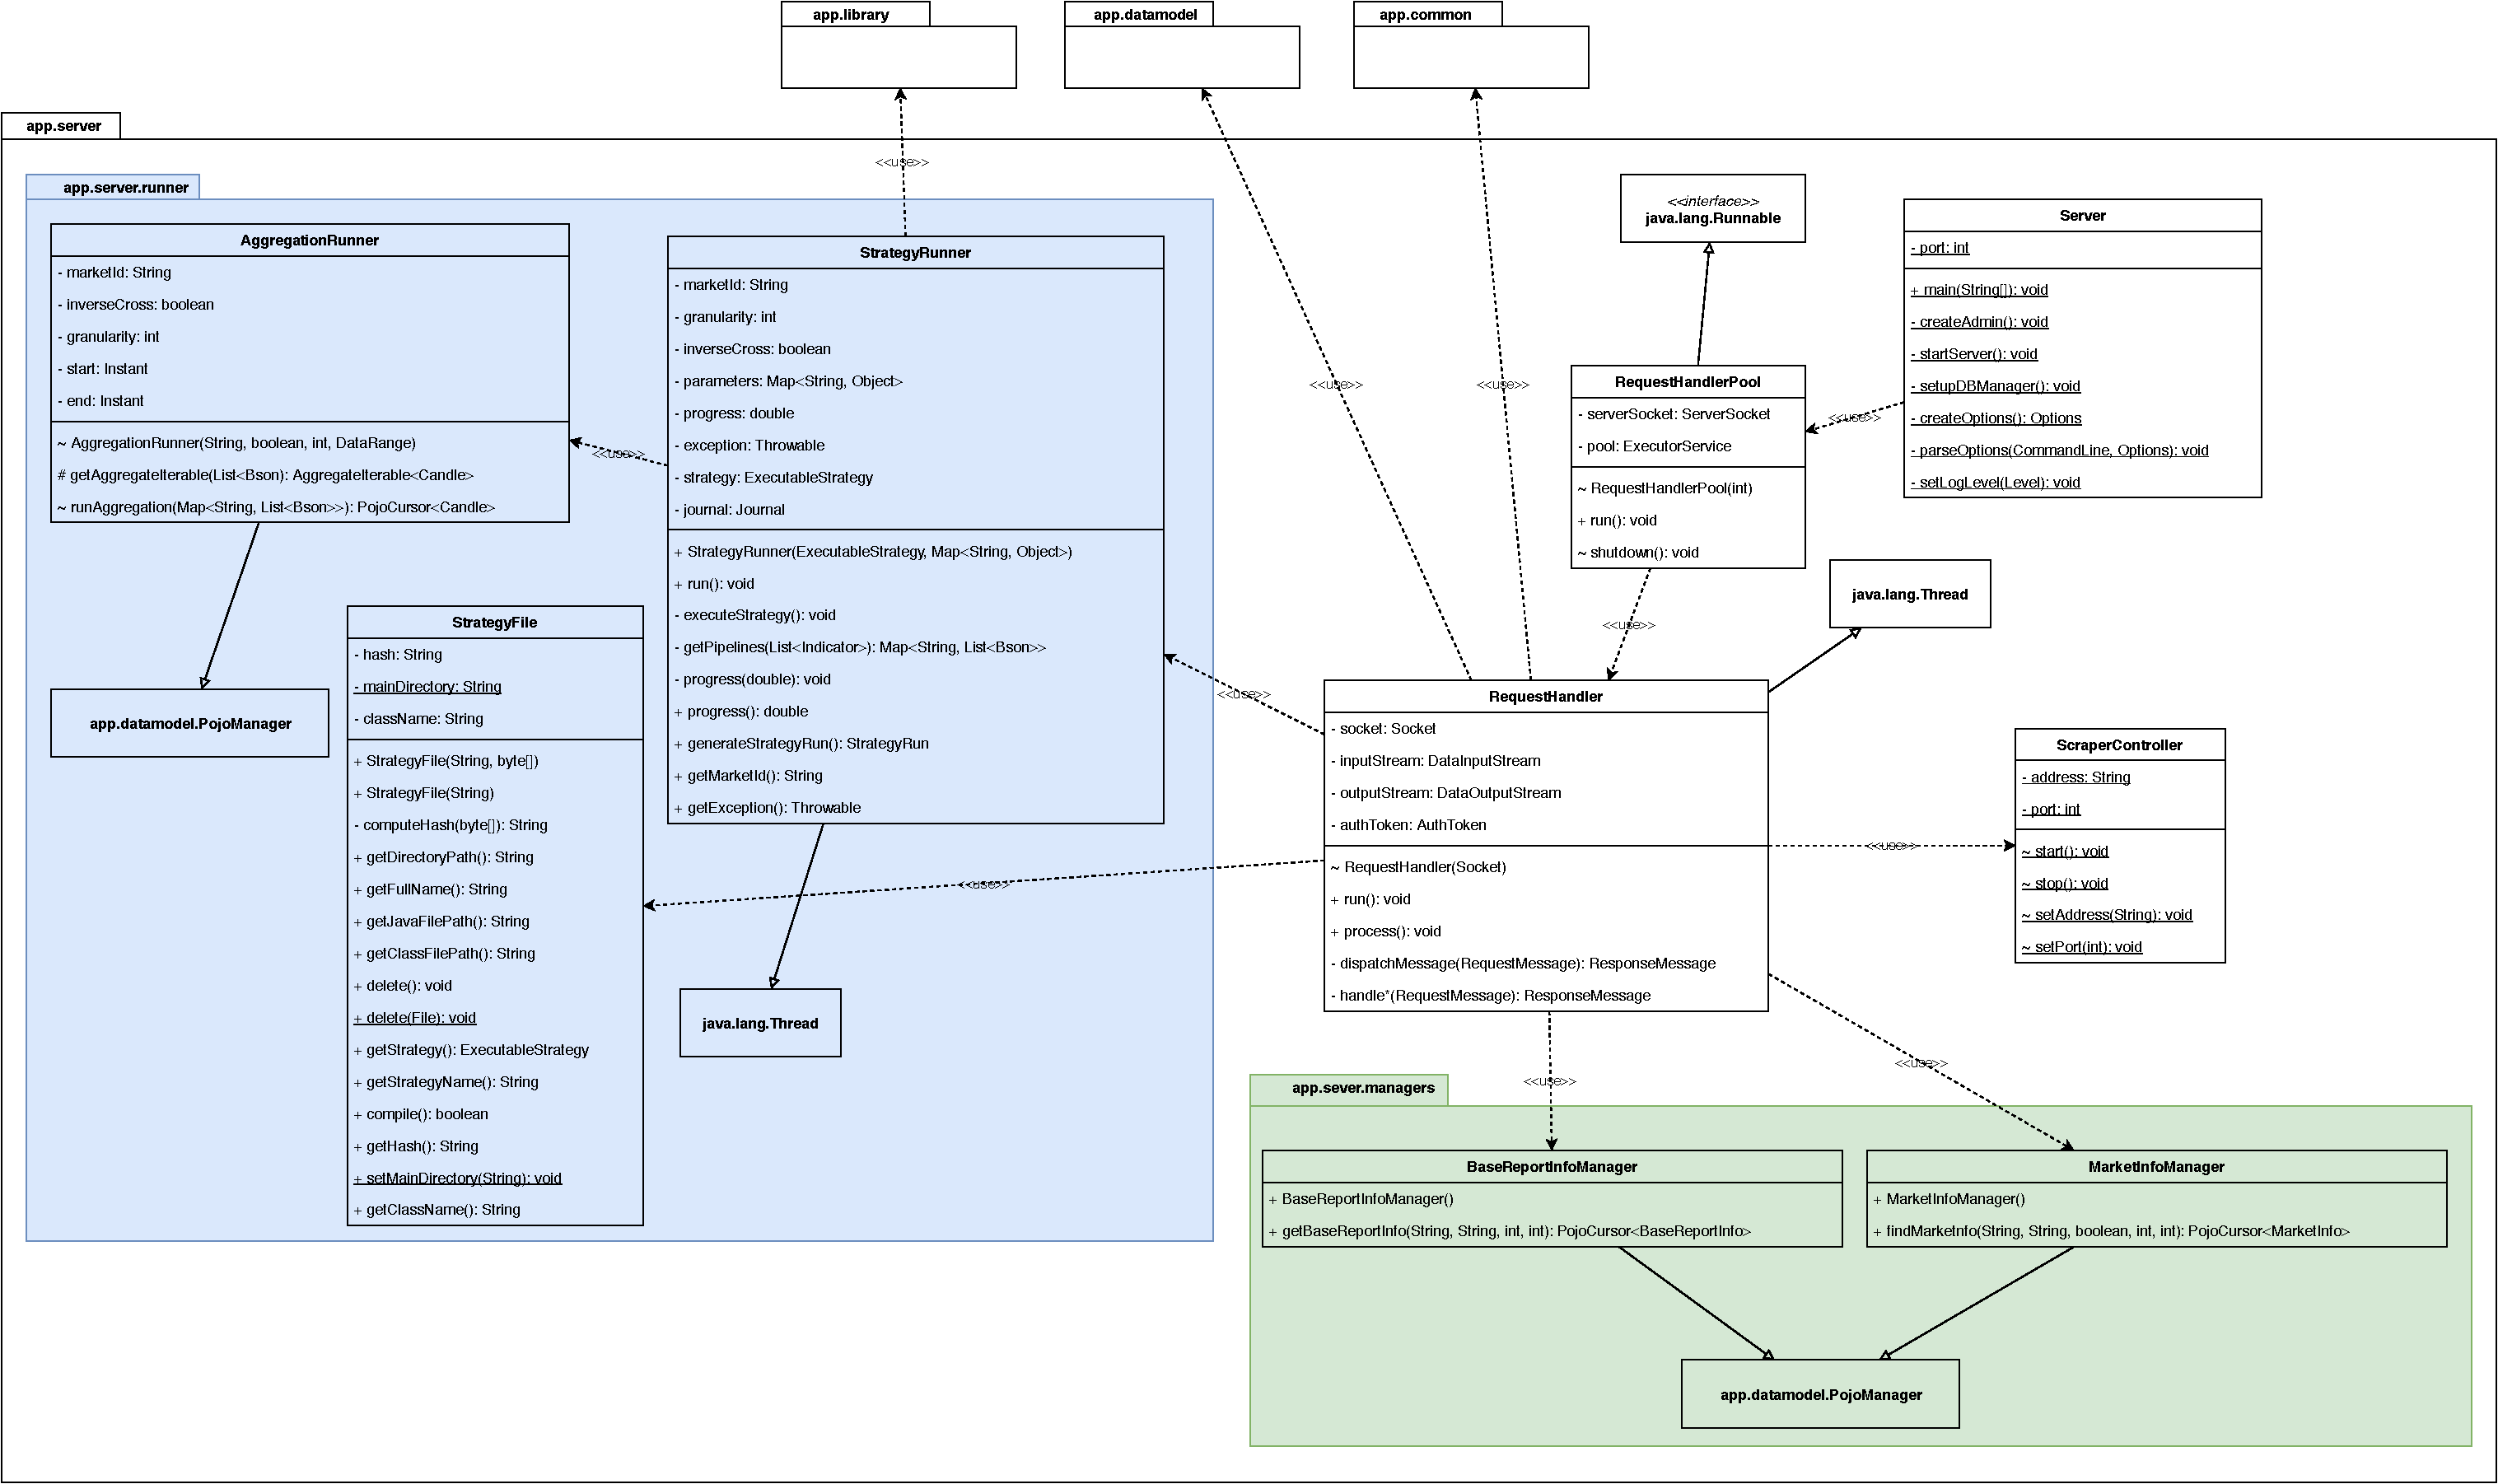
\includegraphics[width=0.8\paperheight]{module-server}
		\caption*{\textbf{Figure~\ref{fig:server}}}
		\captionlistentry{}\label{fig:server}
	\end{figure}
\end{landscape}

\section{Client}\label{sec:client}

The client application is substantially a collection of menus and forms. Each
menus creates a list of entries and when the user selects an entry the
corresponding handler (a method) is called. Forms validate every input that the
user inserts.

The crafting of the requests to submit to the server is made by the
\code{Protocol} class. Beside that, the client only implements presentation
logic.

\begin{landscape}
	\begin{figure}[!h]
		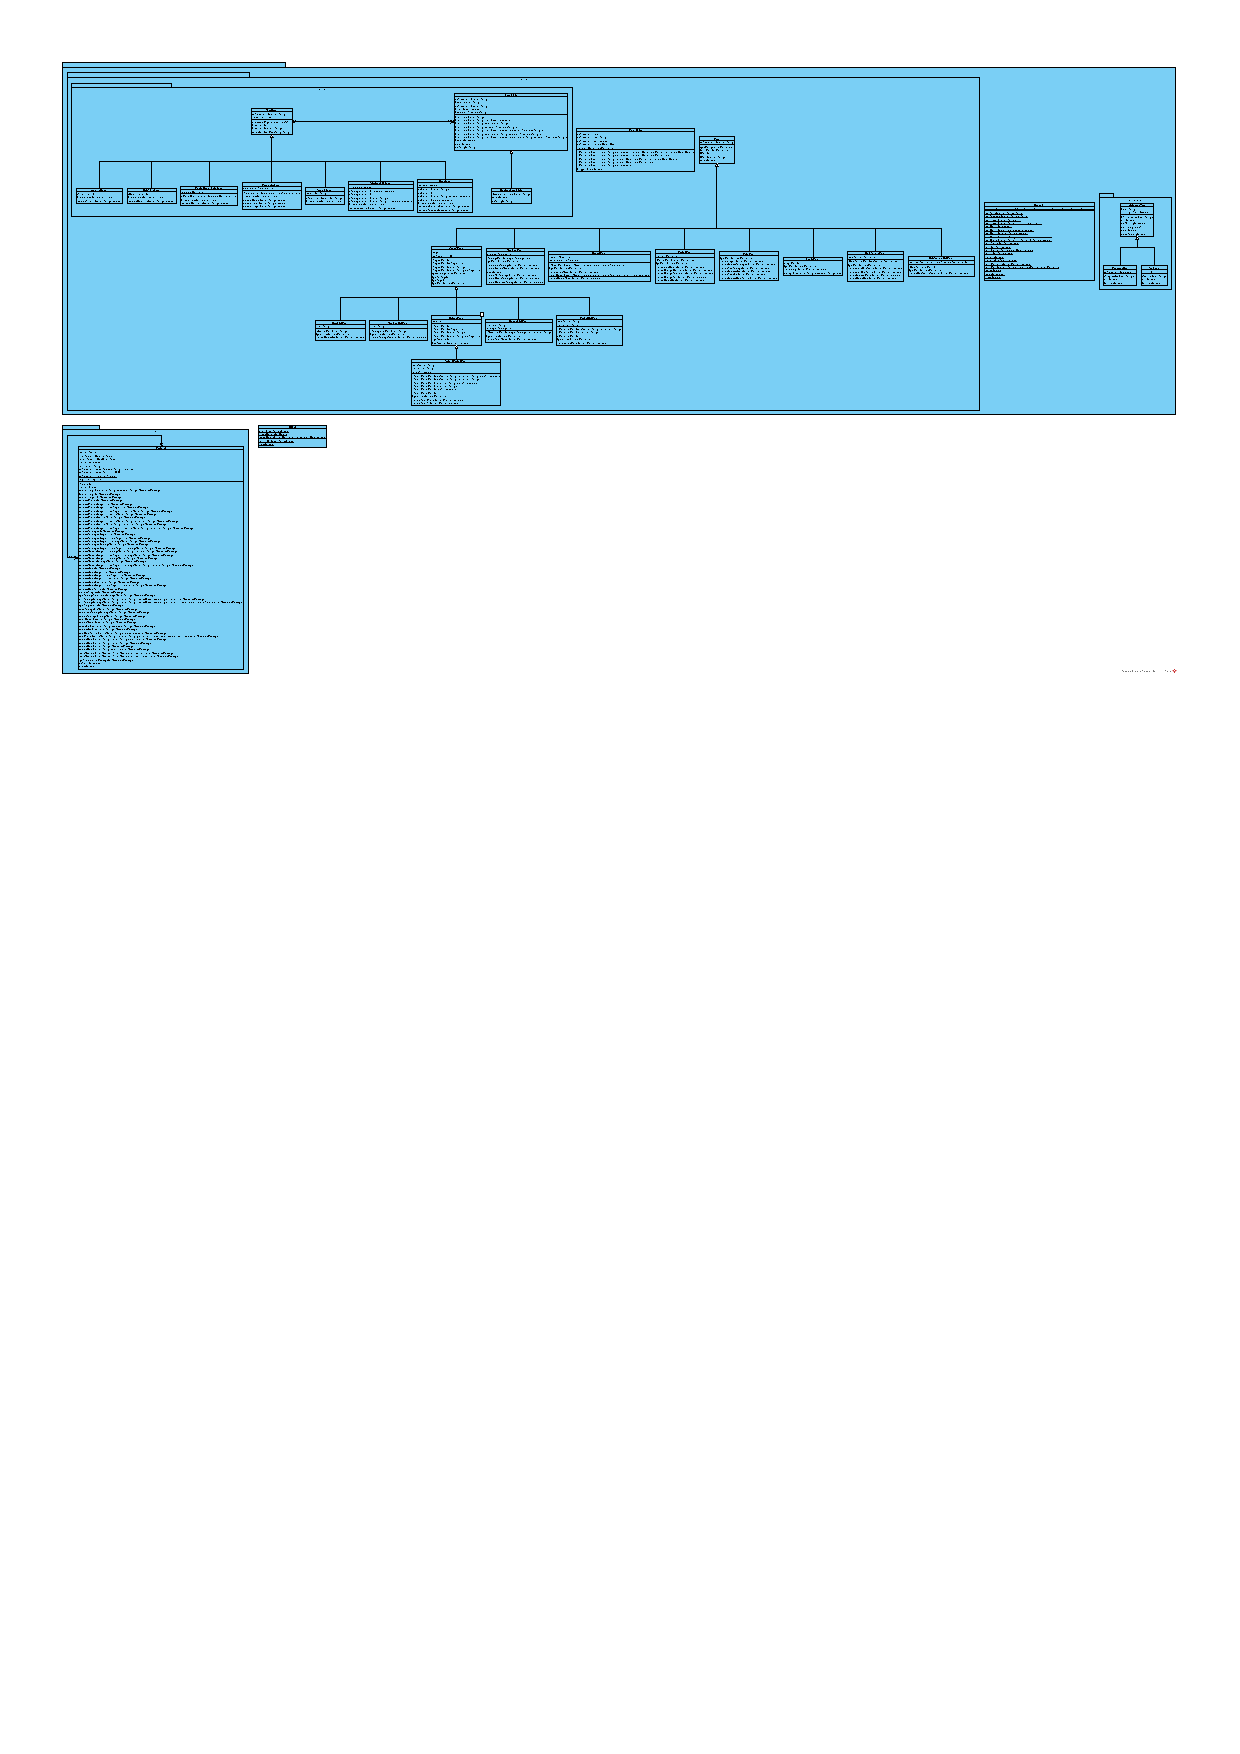
\includegraphics[width=0.8\paperheight]{module-client}
		\caption*{\textbf{Figure~\ref{fig:client}}}
		\captionlistentry{}\label{fig:client}
	\end{figure}
\end{landscape}

\section{Replication and Sharding}\label{sec:distributed}

The application uses replicas to ensure high availability.

All programs that compound the application will always write to the primary
server (as enforced by \mongodb).

The scraper will use the \standout{read preference mode}
\code{primary}, meaning that it will \emph{always} read from the primary server
(if the primary is not online, the read operation will fail). In fact the
scraper needs to be \emph{sure} that the configuration that reads from the
database is the last configuration submitted by the administrator. Moreover,
since the objective of the scraper is to download data and store it in the
database, it would not make sense to run the scraper when the primary server is
not available (the scraper would not be allowed to write to the database).

The server will use the \standout{read preference mode} \code{nearest}, meaning
that it will read from the server with the least network latency. It is in fact
acceptable that some data that the server reads may not be up to date.

To ensure a good load balancing between cluster's servers the \code{Market\-Data}
collection is sharded, because it is the biggest one and it is often read when
running a strategy.

The \code{\_id} field is the shard key since it has a good granularity (so
\mongodb{} can split the documents into a large number of chunks). The field is
hash-indexed, thus the chunks will be randomly distributed across the configured
servers.

\section{Third-party softwares}\label{sec:dependencies}

The following frameworks and libraries are used:
\begin{description}
	\item[Apache Commons CLI v1.4] \textit{(Client, Server)} for parse
		command-line options;
	\item[Gson v2.8.6] \textit{(Scraper)} for JSON deserialization of data
		sources' API responses;
	\item[MongoDB Java Driver v4.0.0] \textit{(Scraper, Server)} for
		handling MongoDB server;
	\item[Retrofit v2.7.2] \textit{(Scraper)} for building HTTP API
		requests;
	\item[XStream v1.4.12] \textit{(All)} for XML
		serialization/deserialization to transmit objects over the
		network.
\end{description}

In the final implementation of the application, newer versions of the
aforementioned dependencies may be used (if they will be released during the
development).

All dependencies are handled with Maven. Other frameworks or libraries may be
added in future.

\section{Further improvements}\label{sec:future}

When a user logs-in with the server, an auth token is created and returned to
the client. From now on, the client resends this token with every request with
the server. This allows for the server to be \standout{stateless} \idest{it does
not need to maintain the user login informations on its memory: when a new
request arrive, it just checks again the database for the validity of the
token}.

With a stateless server, we can also distribute it on multiple servers in order
to ensure high availability of the application and better performance, since it
does not matter which server handles the request when it arrives from the
client.

We may choose to distribute the server program on multiple server machines with
\standout{Docker Swarm}. But since this decision does not impact with the
design, the architecture and the implementation of the application, we postpone
this decision to the future.

